%!TeX root = thesis-main.tex

\begin{figure}[t]
  \centering
  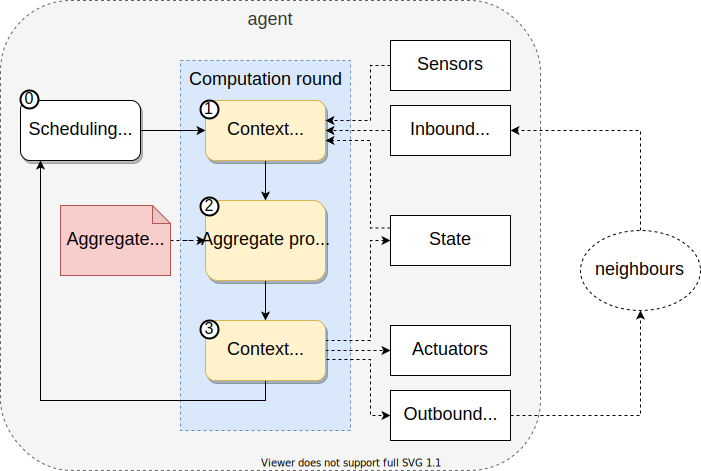
\includegraphics[width=0.9\textwidth]{papers/coordination2022/img/aggregate-agent-control-architecture.pdf}
  \caption[Integration of \ac{RL} within the \ac{ac} control architecture for collective program synthesis]{Integration of \ac{rl} within the \ac{ac} control architecture~\cite{DBLP:journals/jsan/CasadeiAV21}. 
  %
  The \ac{rl} state and reward concepts build upon the context, given by environment and neighbour data. 
  %
  The designer configures action points where learning can improve the aggregate computation. 
  %
  The actions selected by the learned policies will then affect the environment (via actuators) and neighbours (via outbound messages).}
  \label{coordination2022:fig:ac-and-rl}
\end{figure}